% Options for packages loaded elsewhere
\PassOptionsToPackage{unicode}{hyperref}
\PassOptionsToPackage{hyphens}{url}
%
\documentclass[
]{book}
\usepackage{amsmath,amssymb}
\usepackage{lmodern}
\usepackage{iftex}
\ifPDFTeX
  \usepackage[T1]{fontenc}
  \usepackage[utf8]{inputenc}
  \usepackage{textcomp} % provide euro and other symbols
\else % if luatex or xetex
  \usepackage{unicode-math}
  \defaultfontfeatures{Scale=MatchLowercase}
  \defaultfontfeatures[\rmfamily]{Ligatures=TeX,Scale=1}
\fi
% Use upquote if available, for straight quotes in verbatim environments
\IfFileExists{upquote.sty}{\usepackage{upquote}}{}
\IfFileExists{microtype.sty}{% use microtype if available
  \usepackage[]{microtype}
  \UseMicrotypeSet[protrusion]{basicmath} % disable protrusion for tt fonts
}{}
\makeatletter
\@ifundefined{KOMAClassName}{% if non-KOMA class
  \IfFileExists{parskip.sty}{%
    \usepackage{parskip}
  }{% else
    \setlength{\parindent}{0pt}
    \setlength{\parskip}{6pt plus 2pt minus 1pt}}
}{% if KOMA class
  \KOMAoptions{parskip=half}}
\makeatother
\usepackage{xcolor}
\usepackage{color}
\usepackage{fancyvrb}
\newcommand{\VerbBar}{|}
\newcommand{\VERB}{\Verb[commandchars=\\\{\}]}
\DefineVerbatimEnvironment{Highlighting}{Verbatim}{commandchars=\\\{\}}
% Add ',fontsize=\small' for more characters per line
\usepackage{framed}
\definecolor{shadecolor}{RGB}{248,248,248}
\newenvironment{Shaded}{\begin{snugshade}}{\end{snugshade}}
\newcommand{\AlertTok}[1]{\textcolor[rgb]{0.94,0.16,0.16}{#1}}
\newcommand{\AnnotationTok}[1]{\textcolor[rgb]{0.56,0.35,0.01}{\textbf{\textit{#1}}}}
\newcommand{\AttributeTok}[1]{\textcolor[rgb]{0.77,0.63,0.00}{#1}}
\newcommand{\BaseNTok}[1]{\textcolor[rgb]{0.00,0.00,0.81}{#1}}
\newcommand{\BuiltInTok}[1]{#1}
\newcommand{\CharTok}[1]{\textcolor[rgb]{0.31,0.60,0.02}{#1}}
\newcommand{\CommentTok}[1]{\textcolor[rgb]{0.56,0.35,0.01}{\textit{#1}}}
\newcommand{\CommentVarTok}[1]{\textcolor[rgb]{0.56,0.35,0.01}{\textbf{\textit{#1}}}}
\newcommand{\ConstantTok}[1]{\textcolor[rgb]{0.00,0.00,0.00}{#1}}
\newcommand{\ControlFlowTok}[1]{\textcolor[rgb]{0.13,0.29,0.53}{\textbf{#1}}}
\newcommand{\DataTypeTok}[1]{\textcolor[rgb]{0.13,0.29,0.53}{#1}}
\newcommand{\DecValTok}[1]{\textcolor[rgb]{0.00,0.00,0.81}{#1}}
\newcommand{\DocumentationTok}[1]{\textcolor[rgb]{0.56,0.35,0.01}{\textbf{\textit{#1}}}}
\newcommand{\ErrorTok}[1]{\textcolor[rgb]{0.64,0.00,0.00}{\textbf{#1}}}
\newcommand{\ExtensionTok}[1]{#1}
\newcommand{\FloatTok}[1]{\textcolor[rgb]{0.00,0.00,0.81}{#1}}
\newcommand{\FunctionTok}[1]{\textcolor[rgb]{0.00,0.00,0.00}{#1}}
\newcommand{\ImportTok}[1]{#1}
\newcommand{\InformationTok}[1]{\textcolor[rgb]{0.56,0.35,0.01}{\textbf{\textit{#1}}}}
\newcommand{\KeywordTok}[1]{\textcolor[rgb]{0.13,0.29,0.53}{\textbf{#1}}}
\newcommand{\NormalTok}[1]{#1}
\newcommand{\OperatorTok}[1]{\textcolor[rgb]{0.81,0.36,0.00}{\textbf{#1}}}
\newcommand{\OtherTok}[1]{\textcolor[rgb]{0.56,0.35,0.01}{#1}}
\newcommand{\PreprocessorTok}[1]{\textcolor[rgb]{0.56,0.35,0.01}{\textit{#1}}}
\newcommand{\RegionMarkerTok}[1]{#1}
\newcommand{\SpecialCharTok}[1]{\textcolor[rgb]{0.00,0.00,0.00}{#1}}
\newcommand{\SpecialStringTok}[1]{\textcolor[rgb]{0.31,0.60,0.02}{#1}}
\newcommand{\StringTok}[1]{\textcolor[rgb]{0.31,0.60,0.02}{#1}}
\newcommand{\VariableTok}[1]{\textcolor[rgb]{0.00,0.00,0.00}{#1}}
\newcommand{\VerbatimStringTok}[1]{\textcolor[rgb]{0.31,0.60,0.02}{#1}}
\newcommand{\WarningTok}[1]{\textcolor[rgb]{0.56,0.35,0.01}{\textbf{\textit{#1}}}}
\usepackage{longtable,booktabs,array}
\usepackage{calc} % for calculating minipage widths
% Correct order of tables after \paragraph or \subparagraph
\usepackage{etoolbox}
\makeatletter
\patchcmd\longtable{\par}{\if@noskipsec\mbox{}\fi\par}{}{}
\makeatother
% Allow footnotes in longtable head/foot
\IfFileExists{footnotehyper.sty}{\usepackage{footnotehyper}}{\usepackage{footnote}}
\makesavenoteenv{longtable}
\usepackage{graphicx}
\makeatletter
\def\maxwidth{\ifdim\Gin@nat@width>\linewidth\linewidth\else\Gin@nat@width\fi}
\def\maxheight{\ifdim\Gin@nat@height>\textheight\textheight\else\Gin@nat@height\fi}
\makeatother
% Scale images if necessary, so that they will not overflow the page
% margins by default, and it is still possible to overwrite the defaults
% using explicit options in \includegraphics[width, height, ...]{}
\setkeys{Gin}{width=\maxwidth,height=\maxheight,keepaspectratio}
% Set default figure placement to htbp
\makeatletter
\def\fps@figure{htbp}
\makeatother
\setlength{\emergencystretch}{3em} % prevent overfull lines
\providecommand{\tightlist}{%
  \setlength{\itemsep}{0pt}\setlength{\parskip}{0pt}}
\setcounter{secnumdepth}{5}
\usepackage{booktabs}
\usepackage{booktabs}
\usepackage{longtable}
\usepackage{array}
\usepackage{multirow}
\usepackage{wrapfig}
\usepackage{float}
\usepackage{colortbl}
\usepackage{pdflscape}
\usepackage{tabu}
\usepackage{threeparttable}
\usepackage{threeparttablex}
\usepackage[normalem]{ulem}
\usepackage{makecell}
\usepackage{xcolor}
\ifLuaTeX
  \usepackage{selnolig}  % disable illegal ligatures
\fi
\usepackage[]{natbib}
\bibliographystyle{apalike}
\IfFileExists{bookmark.sty}{\usepackage{bookmark}}{\usepackage{hyperref}}
\IfFileExists{xurl.sty}{\usepackage{xurl}}{} % add URL line breaks if available
\urlstyle{same} % disable monospaced font for URLs
\hypersetup{
  pdftitle={Personal Science Cookbook},
  pdfauthor={Friends of Personal Science},
  hidelinks,
  pdfcreator={LaTeX via pandoc}}

\title{Personal Science Cookbook}
\author{Friends of Personal Science}
\date{2022-08-12}

\begin{document}
\maketitle

{
\setcounter{tocdepth}{1}
\tableofcontents
}
\hypertarget{prerequisites}{%
\chapter{Prerequisites}\label{prerequisites}}

\hypertarget{assumptions}{%
\section{Assumptions}\label{assumptions}}

We'll assume some basic tools.

\begin{itemize}
\tightlist
\item
  A spreadsheet like Microsoft Excel
\item
  The programming language R and the associated development environment RStudio
\end{itemize}

A good introduction to R is \href{https://rstudio-education.github.io/hopr/}{Hands On Programming with R}

\begin{Shaded}
\begin{Highlighting}[]
\FunctionTok{library}\NormalTok{(tidyverse)}
\FunctionTok{library}\NormalTok{(lubridate)}
\FunctionTok{library}\NormalTok{(kableExtra)}
\end{Highlighting}
\end{Shaded}

\hypertarget{how-to-edit-this-book}{%
\section{How to edit this book}\label{how-to-edit-this-book}}

This is book written in \textbf{Markdown}. You can use anything that Pandoc's Markdown supports, e.g., a math equation \(a^2 + b^2 = c^2\).

Remember each Rmd file contains one and only one chapter, and a chapter is defined by the first-level heading \texttt{\#}.

To compile this example to PDF, you need XeLaTeX. We recommend TinyTeX (which includes XeLaTeX): \url{https://yihui.org/tinytex/}.

\hypertarget{intro}{%
\chapter{Introduction}\label{intro}}

There's something you want to understand, probably about yourself, maybe something health- or wellness-related, but it might be something about the world around you. The point is that it's a question of deep interest to you, though unlikely in its current form to be of enough interest to involve professionals. You'd like to apply the principles of science --- hypothesis, experiment, analysis --- but you don't know enough of the mechanics to get started.

In other words, like a hungry person in a kitchen full of ingredients, you need a cookbook of recipes that can explain in a step-by-step, repeatable manner, how to go from the raw data around you to some fully-baked insights. That's the purpose of the Personal Science Cookbook. Each ``recipe'' is short and self-contained. Some are more complex than others, but none require any tools or knowledge beyond what is explained in the book.

\hypertarget{the-principles-of-personal-science}{%
\chapter{The Principles of Personal Science}\label{the-principles-of-personal-science}}

Personal Science is about empowering normal people to use the tools of science to help themselves in their daily lives.

When the first microchips enabled desktop computers in the 1970s, people were unsure what to call them.

The word ``mini-computer'' was already taken, referring to a generation of computers that didn't require entire rooms, so the techie engineers who confronted these new machines called them ``microcomputers'', a moniker that lives on in the name for one of the first software companies of that generation, Microsoft.

Some people called them ``hobby computers'', because that seemed to be all they were good for. The most influential early gathering of people using them was called the ``Homebrew Computer Club''. The term ``desktop'' was gaining traction, and inspired later generations that called them ``laptops'', but then the most traditional of all computer companies introduced its first ``IBM PC'', and suddenly the industry had a new term.

It was a ``personal computer'' because, for the first time, it was cheap enough and easy enough for a single individual to use it by him (or her) self. In contrast to all previous generations of computing, everything about the device was intended to be used by a single individual. Even if the computer was shared, only one person would use it at a time, and all design decisions reflected that: a single keyboard, monitor, one power switch. You didn't need a team of people to set up and care for the device --- it was out-of-the-box something that a single person could set up and use.

It's easy to forget how transformative this was at the time. Computers until then were very expensive --- many times more than the cost of a car or even a house. You had to be a large organization --- a university, a business --- to afford one, and even if somebody magically just gave one to you, you'd need a special place to keep it, with highly-trained technicians just to keep it running, and of course even more well-trained engineers and scientists to get it to do anything useful.

\begin{center}\rule{0.5\linewidth}{0.5pt}\end{center}

A similar situation exists today in science. New discoveries are made in large institutions, by teams of high-trained people with access to large, expensive equipment. The discoveries are discussed and shared by specialists who are followed by a cadre of specialized interpreters --- journalists, educators, clinicians --- ~who decipher the new scientific results into lay language and ultimately into face-to-face interaction with the public. Committees meet to discuss takeaways from the expensive and time-consuming research, reaching conclusions that are considered generally acceptable enough to result in new actionable treatments and suggestions for ``normal people''.

This gap between the specialists and the general public, like the gap between mainframe computers and PCs, is eroding thanks to technology.

Actually that's not quite true: the~\emph{potential}~gap between specialists and the general public is eroding. But reality is still different. It's as if PCs had been invented but no software.

The personal computer revolution was about more than simply cheaper devices. The hardware became useful after it spawned an entire industry of dedicated software makers, ~educational experts, consultants and systems integrators,

Professional science

We all think science is great\ldots{}

but what do people mean when they say ``science''?
1. Wonder ~(photos of stars, micrographs, etc.)
2. Technology (photos of roman arch, integrated circuit, moon landing)
3. A way of thinking (photos of ``amateur'' scientists)

It's tempting to assume that the scientific way of thinking is obvious, and maybe even obviously the only way to think rigorously but that's not really true.

Alternatives to the scientific way of thinking:
recipes

My definition of science: a predisposition to the assumption that you're wrong, a nasty mischievous inclination to disbelieve things you can't prove.

A core scientific skill is \emph{curiosity}. ~Always ask ``what if\ldots{}'' ~thinking in hypotheticals

Religion seems like a classic example of unscientific thinking, but even that I'll challenge. What if you're wrong? ~Is there a way to experiment, test it?

Science is:

\begin{itemize}
\tightlist
\item
  Curiosity
\item
  Skepticism : an unending belief that you are wrong

  \begin{itemize}
  \tightlist
  \item
    Low interest in credentials \ldots{} just because you are ``certified'' doesn't mean you know any more than I do.
  \end{itemize}
\item
  Bias toward experiments
\end{itemize}

See \citet{roberts_self-experimentation_2004} for examples.

\hypertarget{methods}{%
\chapter{Methods}\label{methods}}

\hypertarget{what-is-a-dataframe}{%
\section{What is a dataframe?}\label{what-is-a-dataframe}}

Self-collected data is almost always best represented by a table of the variables you want to study and the values that you collected for each of those variables. The most common type of table is a spreadsheet, a specific form of which in Personal Science we refer to as a data table or a \emph{data frame}. Abbreviated ``dataframe'' or often just ``df'', it's a table of values and variables that always has the same form:

\begin{itemize}
\tightlist
\item
  columns are variables: the parameters you want to study
\item
  rows are observations: each incident of data you collected.
\end{itemize}

It's important to get in the habit of this row/column approach to data collection because, as you'll see, all of our tools assume that data will come in a dataframe format.

\hypertarget{is-it-chance-t-test}{%
\section{Is it chance? T-Test}\label{is-it-chance-t-test}}

\textbf{Problem}

You tried an intervention and want to see if it worked. How likely is it that the results were chance?

\textbf{Solution}

One of the simplest tests is a ``T-Test'', sometimes called a ``Student T Test''.

Statisticians use the concept of \emph{P Value} to discuss the how often a result might appear to be significant even when it's not. While this crude measure doesn't describe all the ways something might happen due to chance, generally the lower the P Value, the better. Professional scientists, especially those who understand statistics, will get touchy if you claim a result based purely on P Values, but for Personal Science purposes, it's a good start. There is no ``correct'' cutoff value that can determine the likelihood that something is due to chance alone, but traditionally people assume that anything under 0.05 deserves a closer look.

Here's an example for how to do this in Excel.

Suppose you'd like to know if taking a melotonin supplement will help you sleep longer. You've measured your daily sleep, taking the supplements on some days (the ``intervention'') and not on others (``control'').

A simple spreadsheet might look like this:

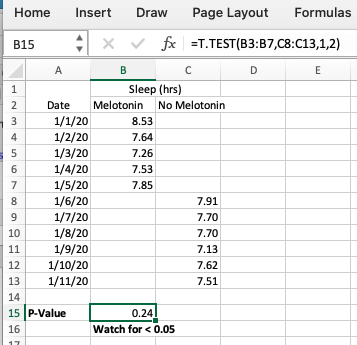
\includegraphics{image-20200828173214548.png}

Track your sleep under two columns: one for nights when you took the supplement, and the other for nights you didn't.

The built-in Excel statistical function \texttt{T.TEST} will calculate the P-Value when you give it two ranges, the ``intervention'' (nights we took melotonin) and the ``control'' (nights without).

See the screenshot for the exact formula in this case:

\texttt{=T.TEST(array1,array2,tails,type)}

Enter a \texttt{1} for \texttt{tails} (because we're only interested in one measurement, sleep) and a \texttt{2} for type (because in this case our samples are not of the same length).

The P Value in this example, \texttt{0.24}, is above \texttt{0.05} and therefore we will assume that any difference in sleep between the nights is due to pure chance.

\hypertarget{rolling-average}{%
\section{Rolling average}\label{rolling-average}}

\textbf{Problem} You want to take the rolling 7-day average of a series of numbers.

\begin{Shaded}
\begin{Highlighting}[]
\NormalTok{headache\_df }\OtherTok{\textless{}{-}} \FunctionTok{read\_csv}\NormalTok{(}\StringTok{"headache{-}variables.csv"}\NormalTok{)}
\NormalTok{headache\_df }\SpecialCharTok{\%\textgreater{}\%} \FunctionTok{head}\NormalTok{() }\SpecialCharTok{\%\textgreater{}\%}\NormalTok{ knitr}\SpecialCharTok{::}\FunctionTok{kable}\NormalTok{()}
\end{Highlighting}
\end{Shaded}

\begin{tabular}{l|l|l|r|r}
\hline
date & headache & icecream & z & wine\\
\hline
2022-05-06 & FALSE & FALSE & 8.161895 & 0\\
\hline
2022-05-07 & FALSE & FALSE & 6.993003 & 0\\
\hline
2022-05-08 & FALSE & FALSE & 5.513575 & 0\\
\hline
2022-05-09 & FALSE & FALSE & 7.565021 & 0\\
\hline
2022-05-10 & FALSE & FALSE & 7.731420 & 0\\
\hline
2022-05-11 & FALSE & FALSE & 7.524007 & 0\\
\hline
\end{tabular}

\textbf{Solution} use the \texttt{rolling()} functions in package \texttt{zoo}:

\begin{Shaded}
\begin{Highlighting}[]
\FunctionTok{library}\NormalTok{(zoo)}
\end{Highlighting}
\end{Shaded}

\begin{verbatim}
## 
## Attaching package: 'zoo'
\end{verbatim}

\begin{verbatim}
## The following objects are masked from 'package:base':
## 
##     as.Date, as.Date.numeric
\end{verbatim}

\begin{Shaded}
\begin{Highlighting}[]
\NormalTok{headache\_df }\SpecialCharTok{\%\textgreater{}\%} 
    \FunctionTok{mutate}\NormalTok{(}\AttributeTok{sleep7A =} \FunctionTok{rollapply}\NormalTok{(z,}
                               \DecValTok{7}\NormalTok{, }
                               \ControlFlowTok{function}\NormalTok{(x) \{x }\OtherTok{=} \FunctionTok{mean}\NormalTok{(x,}\AttributeTok{na.rm =} \ConstantTok{TRUE}\NormalTok{)\},}
                               \AttributeTok{align =} \StringTok{\textquotesingle{}right\textquotesingle{}}\NormalTok{,}
                               \AttributeTok{fill =} \ConstantTok{NA}\NormalTok{)) }\SpecialCharTok{\%\textgreater{}\%} 
  \FunctionTok{tail}\NormalTok{() }\SpecialCharTok{\%\textgreater{}\%}\NormalTok{ knitr}\SpecialCharTok{::}\FunctionTok{kable}\NormalTok{()}
\end{Highlighting}
\end{Shaded}

\begin{tabular}{l|l|l|r|r|r}
\hline
date & headache & icecream & z & wine & sleep7A\\
\hline
2022-08-06 & TRUE & FALSE & 5.648103 & 0 & 7.084293\\
\hline
2022-08-07 & FALSE & TRUE & 8.193874 & 0 & 7.212147\\
\hline
2022-08-08 & FALSE & FALSE & 6.205921 & 0 & 6.950828\\
\hline
2022-08-09 & TRUE & FALSE & 6.623467 & 0 & 6.757966\\
\hline
2022-08-10 & FALSE & FALSE & 7.329287 & 0 & 6.926723\\
\hline
2022-08-11 & FALSE & FALSE & 6.659585 & 2 & 6.854450\\
\hline
\end{tabular}

\hypertarget{applications}{%
\chapter{Applications}\label{applications}}

Some \emph{significant} applications are demonstrated in this chapter.

Let's say you are suffering from unexplained headaches that appear somewhat randomly. You suspect they may be associated with something you eat, but you're not sure, so you've been tracking 14 weeks (98 days) worth of your own data in a spreadsheet that looks like this:

\begin{Shaded}
\begin{Highlighting}[]
\NormalTok{x }\OtherTok{\textless{}{-}} \FunctionTok{tibble}\NormalTok{(}\AttributeTok{date=}\FunctionTok{seq}\NormalTok{(}\AttributeTok{from =} \FunctionTok{today}\NormalTok{()}\SpecialCharTok{{-}}\FunctionTok{weeks}\NormalTok{(}\DecValTok{14}\NormalTok{),}
                     \AttributeTok{by =} \StringTok{"1 day"}\NormalTok{, }\AttributeTok{length.out =} \DecValTok{7}\SpecialCharTok{*}\DecValTok{14}\NormalTok{),}
            \AttributeTok{headache =} \FunctionTok{sample}\NormalTok{(}\FunctionTok{c}\NormalTok{(}\ConstantTok{TRUE}\NormalTok{,}\ConstantTok{FALSE}\NormalTok{), }\DecValTok{7}\SpecialCharTok{*}\DecValTok{14}\NormalTok{,}
                              \AttributeTok{prob =} \FunctionTok{c}\NormalTok{(.}\DecValTok{05}\NormalTok{,.}\DecValTok{95}\NormalTok{),}
                              \AttributeTok{replace =} \ConstantTok{TRUE}\NormalTok{))}

\NormalTok{knitr}\SpecialCharTok{::}\FunctionTok{kable}\NormalTok{( }\FunctionTok{head}\NormalTok{(x) ) }\SpecialCharTok{\%\textgreater{}\%}\NormalTok{ kableExtra}\SpecialCharTok{::}\FunctionTok{kable\_styling}\NormalTok{()}
\end{Highlighting}
\end{Shaded}

\begin{table}
\centering
\begin{tabular}{l|l}
\hline
date & headache\\
\hline
2022-05-06 & FALSE\\
\hline
2022-05-07 & FALSE\\
\hline
2022-05-08 & FALSE\\
\hline
2022-05-09 & FALSE\\
\hline
2022-05-10 & FALSE\\
\hline
2022-05-11 & FALSE\\
\hline
\end{tabular}
\end{table}

\begin{Shaded}
\begin{Highlighting}[]
\FunctionTok{write\_csv}\NormalTok{(x,}\StringTok{"headache{-}days.csv"}\NormalTok{)}
\end{Highlighting}
\end{Shaded}

You can download a copy of this file \href{./headache-days.csv}{here}

With my 14 weeks of data, we can do a few basic calculations:

How frequent are my headaches? Simply total the number of headaches and divide by number of days:

\begin{Shaded}
\begin{Highlighting}[]
\CommentTok{\# headaches per day}
\FunctionTok{sum}\NormalTok{(x}\SpecialCharTok{$}\NormalTok{headache) }\SpecialCharTok{/} \FunctionTok{length}\NormalTok{(x}\SpecialCharTok{$}\NormalTok{headache)}
\end{Highlighting}
\end{Shaded}

\begin{verbatim}
## [1] 0.04081633
\end{verbatim}

\hypertarget{hypothesis}{%
\section{Hypothesis}\label{hypothesis}}

With the data collected and in a nice dataframe format, we can start to ask what might be driving the headaches. One of the first suspected culpritsmight be something that I eat. It's easy to add a few more variables (columns) to the dataframe: (\href{./headache-variables.csv}{download})

\begin{Shaded}
\begin{Highlighting}[]
\NormalTok{z }\OtherTok{\textless{}{-}} \ControlFlowTok{function}\NormalTok{(x)\{}
\NormalTok{m }\OtherTok{=} \ConstantTok{NULL}
\ControlFlowTok{for}\NormalTok{(i }\ControlFlowTok{in} \DecValTok{1}\SpecialCharTok{:}\DecValTok{14}\NormalTok{)\{}
\NormalTok{  m }\OtherTok{=} \FunctionTok{c}\NormalTok{(}\FunctionTok{c}\NormalTok{(}\FunctionTok{rep}\NormalTok{(}\DecValTok{0}\NormalTok{,}\DecValTok{6}\NormalTok{),}
              \FunctionTok{floor}\NormalTok{(}\FunctionTok{runif}\NormalTok{(}\DecValTok{1}\NormalTok{,}\AttributeTok{min=}\DecValTok{0}\NormalTok{,}\AttributeTok{max=}\DecValTok{3}\NormalTok{))),}
\NormalTok{        m)}
\NormalTok{\}}

\NormalTok{m}
\NormalTok{\}}
\NormalTok{x }\OtherTok{\textless{}{-}} \FunctionTok{tibble}\NormalTok{(}\AttributeTok{date=}\FunctionTok{seq}\NormalTok{(}\AttributeTok{from =} \FunctionTok{today}\NormalTok{()}\SpecialCharTok{{-}}\FunctionTok{weeks}\NormalTok{(}\DecValTok{14}\NormalTok{),}
                     \AttributeTok{by =} \StringTok{"1 day"}\NormalTok{, }\AttributeTok{length.out =} \DecValTok{7}\SpecialCharTok{*}\DecValTok{14}\NormalTok{),}
            \AttributeTok{headache =} \FunctionTok{sample}\NormalTok{(}\FunctionTok{c}\NormalTok{(}\ConstantTok{TRUE}\NormalTok{,}\ConstantTok{FALSE}\NormalTok{), }\DecValTok{7}\SpecialCharTok{*}\DecValTok{14}\NormalTok{,}
                              \AttributeTok{prob =} \FunctionTok{c}\NormalTok{(.}\DecValTok{05}\NormalTok{,.}\DecValTok{95}\NormalTok{),}
                              \AttributeTok{replace =} \ConstantTok{TRUE}\NormalTok{),}
            \AttributeTok{icecream =} \FunctionTok{sample}\NormalTok{(}\FunctionTok{c}\NormalTok{(}\ConstantTok{TRUE}\NormalTok{,}\ConstantTok{FALSE}\NormalTok{), }\DecValTok{7}\SpecialCharTok{*}\DecValTok{14}\NormalTok{,}
                              \AttributeTok{prob =} \FunctionTok{c}\NormalTok{(.}\DecValTok{10}\NormalTok{,.}\DecValTok{90}\NormalTok{),}
                              \AttributeTok{replace =} \ConstantTok{TRUE}\NormalTok{),}
            \AttributeTok{z =} \FunctionTok{runif}\NormalTok{(}\DecValTok{7}\SpecialCharTok{*}\DecValTok{14}\NormalTok{, }\AttributeTok{min =} \SpecialCharTok{{-}}\FloatTok{2.5}\NormalTok{, }\AttributeTok{max =}\NormalTok{ .}\DecValTok{5}\NormalTok{) }\SpecialCharTok{+} \DecValTok{8}\NormalTok{,}
            \AttributeTok{wine =} \FunctionTok{z}\NormalTok{(}\DecValTok{0}\NormalTok{))}

\NormalTok{knitr}\SpecialCharTok{::}\FunctionTok{kable}\NormalTok{( }\FunctionTok{head}\NormalTok{(x,}\DecValTok{10}\NormalTok{), }\AttributeTok{digits =} \DecValTok{2}\NormalTok{) }\SpecialCharTok{\%\textgreater{}\%}
\NormalTok{  kableExtra}\SpecialCharTok{::}\FunctionTok{kable\_styling}\NormalTok{(}\AttributeTok{bootstrap\_options =} \FunctionTok{c}\NormalTok{(}\StringTok{"striped"}\NormalTok{, }\StringTok{"hover"}\NormalTok{, }\StringTok{"condensed"}\NormalTok{))}
\end{Highlighting}
\end{Shaded}

\begin{table}
\centering
\begin{tabular}{l|l|l|r|r}
\hline
date & headache & icecream & z & wine\\
\hline
2022-05-06 & TRUE & FALSE & 7.16 & 0\\
\hline
2022-05-07 & FALSE & FALSE & 8.32 & 0\\
\hline
2022-05-08 & FALSE & FALSE & 8.11 & 0\\
\hline
2022-05-09 & FALSE & FALSE & 5.97 & 0\\
\hline
2022-05-10 & FALSE & FALSE & 7.76 & 0\\
\hline
2022-05-11 & FALSE & FALSE & 5.66 & 0\\
\hline
2022-05-12 & FALSE & FALSE & 8.04 & 2\\
\hline
2022-05-13 & FALSE & FALSE & 8.29 & 0\\
\hline
2022-05-14 & TRUE & FALSE & 6.51 & 0\\
\hline
2022-05-15 & FALSE & FALSE & 6.02 & 0\\
\hline
\end{tabular}
\end{table}

\begin{Shaded}
\begin{Highlighting}[]
\FunctionTok{write\_csv}\NormalTok{(x,}\StringTok{"headache{-}variables.csv"}\NormalTok{)}
\end{Highlighting}
\end{Shaded}

\begin{itemize}
\tightlist
\item
  \texttt{headache}: a day when I have a headache
\item
  \texttt{icecream}: did I eat ice cream that day?
\item
  \texttt{wine}: Number of glasses of wine I drank.
\item
  \texttt{z}: Number of hours I slept that day.
\end{itemize}

Based on the data collected so far, can I make any guesses about what might be driving my headaches?

The most obvious place to check is whether I see any patterns on the days when I have headaches. Let's filter for headache days only:

\begin{Shaded}
\begin{Highlighting}[]
\NormalTok{x }\SpecialCharTok{\%\textgreater{}\%} \FunctionTok{filter}\NormalTok{(headache)  }\SpecialCharTok{\%\textgreater{}\%}\NormalTok{ kableExtra}\SpecialCharTok{::}\FunctionTok{kable}\NormalTok{() }\SpecialCharTok{\%\textgreater{}\%} 
\NormalTok{  kableExtra}\SpecialCharTok{::}\FunctionTok{kable\_styling}\NormalTok{(}\AttributeTok{bootstrap\_options =} \FunctionTok{c}\NormalTok{(}\StringTok{"striped"}\NormalTok{, }\StringTok{"hover"}\NormalTok{, }\StringTok{"condensed"}\NormalTok{))}
\end{Highlighting}
\end{Shaded}

\begin{table}
\centering
\begin{tabular}{l|l|l|r|r}
\hline
date & headache & icecream & z & wine\\
\hline
2022-05-06 & TRUE & FALSE & 7.164881 & 0\\
\hline
2022-05-14 & TRUE & FALSE & 6.508955 & 0\\
\hline
2022-06-26 & TRUE & FALSE & 7.464869 & 0\\
\hline
2022-07-11 & TRUE & FALSE & 6.910989 & 0\\
\hline
2022-07-20 & TRUE & FALSE & 5.665490 & 0\\
\hline
\end{tabular}
\end{table}

But maybe the headache takes a day or two to kick in. We can divide the data by week and see if we can spot any patterns in headache frequency:

\begin{Shaded}
\begin{Highlighting}[]
\NormalTok{x }\SpecialCharTok{\%\textgreater{}\%} \FunctionTok{group\_by}\NormalTok{(}\AttributeTok{week =} \FunctionTok{ntile}\NormalTok{(date,}\DecValTok{7}\NormalTok{)) }\SpecialCharTok{\%\textgreater{}\%} 
  \FunctionTok{summarise}\NormalTok{(}\AttributeTok{headaches =} \FunctionTok{sum}\NormalTok{(headache),}
            \AttributeTok{alcohol =} \FunctionTok{sum}\NormalTok{(wine),}
            \AttributeTok{icecream =} \FunctionTok{sum}\NormalTok{(icecream))  }\SpecialCharTok{\%\textgreater{}\%}\NormalTok{ kableExtra}\SpecialCharTok{::}\FunctionTok{kable}\NormalTok{() }\SpecialCharTok{\%\textgreater{}\%} 
\NormalTok{  kableExtra}\SpecialCharTok{::}\FunctionTok{kable\_styling}\NormalTok{(}\AttributeTok{bootstrap\_options =} \FunctionTok{c}\NormalTok{(}\StringTok{"striped"}\NormalTok{, }\StringTok{"hover"}\NormalTok{, }\StringTok{"condensed"}\NormalTok{))}
\end{Highlighting}
\end{Shaded}

\begin{table}
\centering
\begin{tabular}{r|r|r|r}
\hline
week & headaches & alcohol & icecream\\
\hline
1 & 2 & 2 & 0\\
\hline
2 & 0 & 1 & 2\\
\hline
3 & 0 & 2 & 0\\
\hline
4 & 1 & 1 & 3\\
\hline
5 & 1 & 2 & 3\\
\hline
6 & 1 & 3 & 0\\
\hline
7 & 0 & 1 & 6\\
\hline
\end{tabular}
\end{table}

Buy simply eye-balling the data this way, you might see a pattern. For example, you might spot a week or two with an unusually large number of headaches and notice those weeks are accompanied by an unusually large consumption of some particular food.

But how do you know you're not just guessing? What \emph{looks} like a pattern might be a coincidence. To find out with more certainty, we will apply some statistics.

\hypertarget{t-testing}{%
\section{T-Testing}\label{t-testing}}

The simplest test is called a ``T Test''. This is a formula that can compare two equal-sized lists of numbers and return the probability that any differences between the two are the result of chance.

What are the chances that the number of headaches per week is related to the amount of ice cream I eat per week?

If there were a relationship between ice cream and headaches each week, I'd expect that over the weeks in this period, the total number of headaches and the total number of ice cream days should be roughly equal.

\begin{Shaded}
\begin{Highlighting}[]
\NormalTok{x\_week }\OtherTok{\textless{}{-}}\NormalTok{ x }\SpecialCharTok{\%\textgreater{}\%} \FunctionTok{group\_by}\NormalTok{(}\AttributeTok{week =} \FunctionTok{ntile}\NormalTok{(date,}\DecValTok{7}\NormalTok{)) }\SpecialCharTok{\%\textgreater{}\%} 
  \FunctionTok{summarise}\NormalTok{(}\AttributeTok{headaches =} \FunctionTok{sum}\NormalTok{(headache),}
            \AttributeTok{alcohol =} \FunctionTok{sum}\NormalTok{(wine),}
            \AttributeTok{icecream =} \FunctionTok{sum}\NormalTok{(icecream)) }
\NormalTok{x\_week }\SpecialCharTok{\%\textgreater{}\%}\NormalTok{ kableExtra}\SpecialCharTok{::}\FunctionTok{kable}\NormalTok{() }\SpecialCharTok{\%\textgreater{}\%}
\NormalTok{  kableExtra}\SpecialCharTok{::}\FunctionTok{kable\_styling}\NormalTok{(}\AttributeTok{bootstrap\_options =} \FunctionTok{c}\NormalTok{(}\StringTok{"striped"}\NormalTok{, }\StringTok{"hover"}\NormalTok{, }\StringTok{"condensed"}\NormalTok{)) }
\end{Highlighting}
\end{Shaded}

\begin{table}
\centering
\begin{tabular}{r|r|r|r}
\hline
week & headaches & alcohol & icecream\\
\hline
1 & 2 & 2 & 0\\
\hline
2 & 0 & 1 & 2\\
\hline
3 & 0 & 2 & 0\\
\hline
4 & 1 & 1 & 3\\
\hline
5 & 1 & 2 & 3\\
\hline
6 & 1 & 3 & 0\\
\hline
7 & 0 & 1 & 6\\
\hline
\end{tabular}
\end{table}

\begin{Shaded}
\begin{Highlighting}[]
\FunctionTok{with}\NormalTok{(x\_week, }\FunctionTok{t.test}\NormalTok{(headaches,icecream))[[}\StringTok{"p.value"}\NormalTok{]]}
\end{Highlighting}
\end{Shaded}

\begin{verbatim}
## [1] 0.1907322
\end{verbatim}

By convention, a p-value less than 0.5 is considered statistically significant. While this is not a hard and fast rule, it's often a good place to start. A p-value greater than this is almost certainly due to chance.

\hypertarget{data-visualization}{%
\section{Data visualization}\label{data-visualization}}

The first step in a more sophisticated analysis is to plot the data to see if we can spot any particular patterns.

\begin{Shaded}
\begin{Highlighting}[]
\NormalTok{x\_week }\SpecialCharTok{\%\textgreater{}\%} \FunctionTok{pivot\_longer}\NormalTok{(}\AttributeTok{names\_to =} \StringTok{"activity"}\NormalTok{,}
                        \AttributeTok{values\_to =} \StringTok{"amount"}\NormalTok{,}
                        \AttributeTok{cols =}\NormalTok{ alcohol}\SpecialCharTok{:}\NormalTok{icecream ) }\SpecialCharTok{\%\textgreater{}\%} 
  \FunctionTok{ggplot}\NormalTok{(}\FunctionTok{aes}\NormalTok{(}\AttributeTok{x=}\NormalTok{week,}\AttributeTok{y=}\NormalTok{headaches)) }\SpecialCharTok{+}
  \FunctionTok{geom\_bar}\NormalTok{(}\FunctionTok{aes}\NormalTok{(}\AttributeTok{x=}\NormalTok{week,}\AttributeTok{y=}\NormalTok{amount, }\AttributeTok{fill =}\NormalTok{ activity),}
           \AttributeTok{position =} \StringTok{"dodge"}\NormalTok{,}
           \AttributeTok{stat =} \StringTok{"identity"}\NormalTok{) }\SpecialCharTok{+}
  \FunctionTok{geom\_line}\NormalTok{(}\FunctionTok{aes}\NormalTok{(}\AttributeTok{x=}\NormalTok{week,}\AttributeTok{y=}\NormalTok{headaches))}
\end{Highlighting}
\end{Shaded}

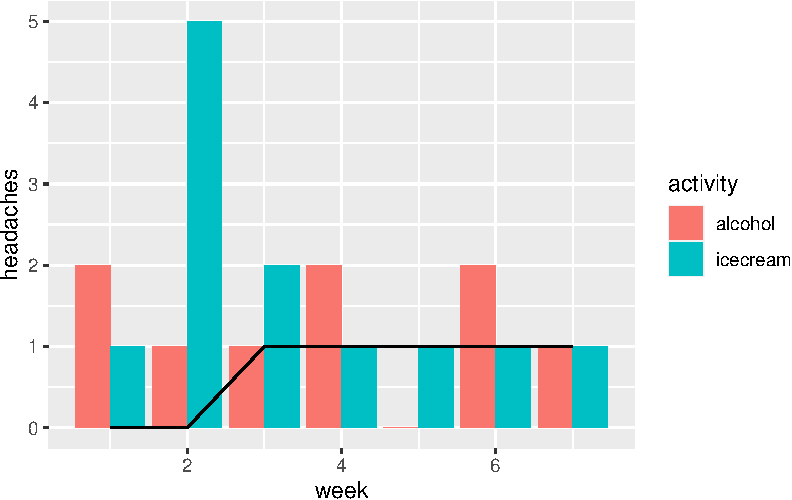
\includegraphics{cookbook_files/figure-latex/plotheadaches-1.pdf}

\hypertarget{example-two}{%
\section{Example two}\label{example-two}}

\hypertarget{final-words}{%
\chapter{Final Words}\label{final-words}}

We have finished a nice book.

  \bibliography{book.bib,packages.bib}

\end{document}
